\section{Learning What High-Level Plan to Refine}
\subsection{Significance}
Recall that in Alg.\,\ref{alg:complete}, the high level has
a two-tiered decision to make: 1) which node in the {\sc prg} to visit
next, and 2) whether to attempt to refine this node or generate
failure information from it. These decisions are encoded in the
routines \textsc{NDGetNextNode} and \textsc{NDChoice} in the outermost loops. Making these
decisions intelligently is critical to good performance. 

For example, consider a pick-place domain. Different sampled grasping
poses may cause different obstruction errors to be propagated back up to
the task planner. \figref{fig:hlsearch} illustrates two different
failures, one of which generates a larger number of obstructions. The
{\sc prg} contains plans to remedy both of these issues; however, one
will take much longer to refine than the other. An effective heuristic
would allow us to allocate more search effort for the promising
plan. In this section, we describe a method to learn one such
heuristic.

\subsection{Approach}
Direct application of {\sc rl} at the high level is difficult for two reasons: 1) the
space of potential high-level plans is very large and reward are
sparse; 2) actions take a long time to `execute' as they often require
motion planning. These combine to make the learning problem quite
challenging, so we use {\sc irl} with expert demonstrations to
train heuristics.

The heuristics are trained to trade off the computation time from
refining a plan with that of generating a plan correction and adding a
new plan to the {\sc prg}. We use $u$ to represent the selected node
and $m$ the mode to apply (either trying to refine the node or
quickly generating failure information).

We encode geometric features of a current plan refinement in a feature
vector $f(u).$ We train separate weights to estimate the utility of
each mode. We do this by stacking two copies of the features and using
an indicator to zero out the top or bottom half: $f((u, m))
= \begin{bmatrix} f(u) \\ f(u) \end{bmatrix}^\top \begin{bmatrix} 1 -
  m \\ m \end{bmatrix}.\vspace{2pt}$ 

We obtain human-demonstrated trajectories (sequences of actions $(u,
m)^{*}$) that intelligently navigate the {\sc prg}. We solve the
following maximum-margin optimization~\cite{taskar2005learning} to
recover a set of weights so that the expert's demonstration is
(approximately) optimal:
\begin{align*}
&\min_{w, \xi_i \geq 0} & ||w||^2 + C \sum_i \xi_i\\
&\text{s.t.} & w^{\top}f^*_i \geq w^{\top}f_{ij} + 1 - \xi_{i}\ \forall i, j \ .
\end{align*}

The $i$ iterate over the demonstrated trajectories and the $j$ iterate
over possible actions. The $\xi_{i}$ are slack variables that ensure
a solution always exists. $C$ is a regularization parameter that
controls overfitting. At test time, we follow the policy encoded by
$w$, picking the highest-scoring action at each step.

A single round of this approach often fails. The graphs generated by a
human expert tend to look very different from those generated by
the learned policy. We thus use dataset
aggregation~\cite{dagger}, a general approach to this problem where
the expert provides new demonstrations on a set of states generated by
executing the learned policy.

\begin{figure}[t]
  \centering
    \noindent
    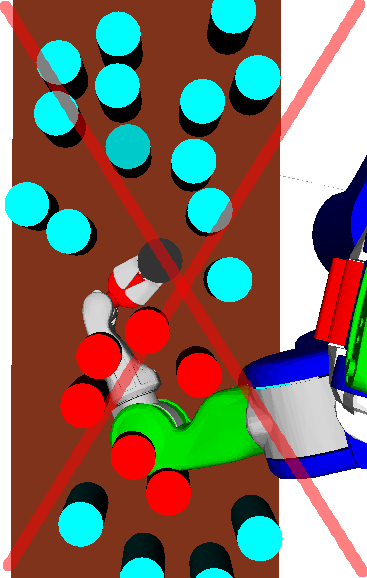
\includegraphics[scale=0.17, angle=270]{images/grasp_teaser_bad.png}
    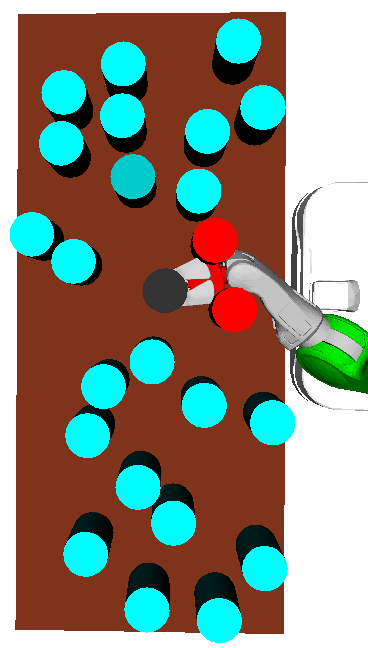
\includegraphics[scale=0.17, angle=270]{images/grasp_teaser_good.png}
  \caption{\small{In this problem, the goal is to grasp the black
      can. Obstructions make it so that this is not immediately possible; however, which
      obstructions are moved will have a big impact on how long it
      takes to find a solution (i.e., 6 obstructions in the left image
      versus 2 obstructions in the right image). Each of these failures
      generates a new node in the plan refinement graph. We learn
      heuristics from expert demonstrations that allow the search to
      focus on the promising nodes in the graph.}}
  \label{fig:hlsearch}
\end{figure}

% \begin{figure}[t]
%   \centering
%     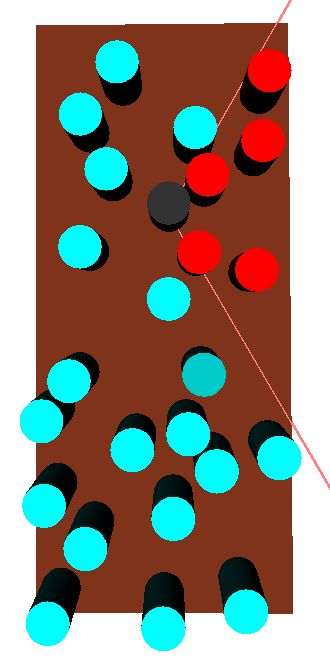
\includegraphics[scale=0.3,angle=90]{images/feature_cone.png}
%   \caption{\small{If the target object to be grasped is the black can, we consider the objects
% whose centers lie in a cone from angles $-\frac{\pi}{3}$ to $\frac{\pi}{3}$ toward the closest table edge in
% our feature computations. These objects are shown here in red.}}
%   \label{fig:cone}
% \end{figure}
